\documentclass[crop]{standalone}

\usepackage{tikz}
\usetikzlibrary{calc}

\tikzset {
  potato style/.style = {
    thick,
    fill=black!5,
    opacity=0.9,
    draw=black
  },
  pics/potato/.style args = {#1 #2 #3}{
    code = {
      \path ({-1.1*#1*(1+#3)}, {-1.1*#1*#2*(1+#3)}) rectangle ({1.1*#1*(1+#3)}, {1.1*#1*#2*(1+#3)});
      \filldraw[potato style, pic actions] plot [domain=0:360, samples=50]
      ({(1+0.5*#3*sin(2*\x+20))*(1+#3*sin(\x))*(1.0*#1*cos(\x))},
       {(1+0.5*#3*sin(2*\x+20))*(1+#3*sin(\x))*( #2*#1*sin(\x))})
       --cycle;
    }
  }
}

\usepackage{amsmath}
\newcommand{\B}{\mathcal{B}}
\newcommand{\F}{\boldsymbol{F}}
\newcommand{\e}{\mathrm{e}}
\renewcommand{\v}{\mathrm{v}}


\begin{document}

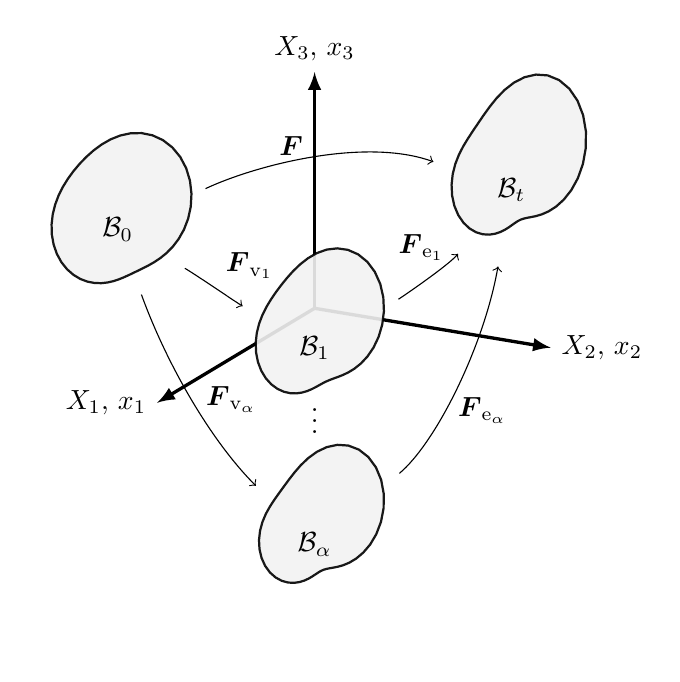
\begin{tikzpicture}[scale=1.0]

% --- Axes ---
\draw[-latex,very thick] (0,0) -- ( 0, 3.0) node[above] {$X_3,\,x_3$};
\draw[-latex,very thick] (0,0) -- ( 3,-0.5) node[right] {$X_2,\,x_2$};
\draw[-latex,very thick] (0,0) -- (-2,-1.2) node[left] {$X_1,\,x_1$};

\coordinate (B0) at (-2.5, 1  );
\coordinate (Bt) at ( 2.5, 1.5);
\coordinate (B1) at ( 0  ,-0.5);
\coordinate (B2) at ( 0  ,-3.0);

\pic at (B0) {potato={0.8 1.2 0.3}};
\pic at (Bt) {potato={0.7 1.4 0.5}};
\pic at (B1) {potato={0.7 1.3 0.4}};
\pic at (B2) {potato={0.65 1.3 0.5}};

\node at (B0) {$\B_0$};
\node at (Bt) {$\B_t$};
\node at (B1) {$\B_1$};
\node at (B2) {$\B_\alpha$};
\path (B1) --node[midway, above=1pt] {$\vdots$} (B2);

\draw[->, shorten <=35pt, shorten >=30pt]
  (B0) to[out=25, in=160] node[midway, above left] {$\F$} (Bt);
\draw[->, shorten <=28pt, shorten >=30pt]
  (B0) to[out=330, in=150] node[midway, above right] {$\F_{\v_1}$} (B1);
\draw[->, shorten <=25pt, shorten >=30pt]
  (B0) to[out=290, in=135] node[midway, right] {$\F_{\v_\alpha}$} (B2);
\draw[->, shorten <=35pt, shorten >=30pt]
  (B1) to[out=30, in=230] node[midway, above=3pt] {$\F_{\e_1}$} (Bt);
\draw[->, shorten <=40pt, shorten >=28pt]
  (B2) to[out=40, in=260] node[midway, below right] {$\F_{\e_\alpha}$} (Bt);

\end{tikzpicture}

\end{document}
